%%%%%%%%%%%%%%%%%%%%%%%%%%%%%%%%%%%%%%%%%
% The Legrand Orange Book
% LaTeX Template
% Version 2.1.1 (14/2/16)
%
% This template has been downloaded from:
% http://www.LaTeXTemplates.com
%
% Original author:
% Mathias Legrand (legrand.mathias@gmail.com) with modifications by:
% Vel (vel@latextemplates.com)
%
% License:
% CC BY-NC-SA 3.0 (http://creativecommons.org/licenses/by-nc-sa/3.0/)
%
% Compiling this template:
% This template uses biber for its bibliography and makeindex for its index.
% When you first open the template, compile it from the command line with the 
% commands below to make sure your LaTeX distribution is configured correctly:
%
% 1) pdflatex main
% 2) makeindex main.idx -s StyleInd.ist
% 3) biber main
% 4) pdflatex main x 2
%
% After this, when you wish to update the bibliography/index use the appropriate
% command above and make sure to compile with pdflatex several times 
% afterwards to propagate your changes to the document.
%
% This template also uses a number of packages which may need to be
% updated to the newest versions for the template to compile. It is strongly
% recommended you update your LaTeX distribution if you have any
% compilation errors.
%
% Important note:
% Chapter heading images should have a 2:1 width:height ratio,
% e.g. 920px width and 460px height.
%
%%%%%%%%%%%%%%%%%%%%%%%%%%%%%%%%%%%%%%%%%

%----------------------------------------------------------------------------------------
%	PACKAGES AND OTHER DOCUMENT CONFIGURATIONS
%----------------------------------------------------------------------------------------

\documentclass[11pt,fleqn]{book} % Default font size and left-justified equations

\usepackage{ifthen} 
\newboolean{VersionProf}
\setboolean{VersionProf}{false}

\usepackage{wasysym}
\usepackage{esint} % various fancy integral symbols
\usepackage{tikz}
\usepackage{tikz-3dplot}
\usepackage{pgfplots}
\pgfplotsset{compat=1.17}
\usetikzlibrary{patterns}
\usepackage{tkz-euclide} 
\usepackage{mathtools}
\usepackage{xurl}
\usepackage[version=4,arrows=pgf-filled,
textfontname=sffamily,
mathfontname=mathsf]{mhchem}
\usepackage{gensymb}
\usepackage{tabularray}
\usepackage{csquotes}

\usepackage[french]{babel}
\usepackage{dingbat}

\usepackage{environ}
\usepackage{wrapfig}

\NewEnviron{solution}{%
    \ifthenelse{\boolean{VersionProf}}{\begin{solutionA}
        \BODY%*
        \end{solutionA}
    }{%
        \relax%
    }%
}%

\usetikzlibrary {arrows.meta} 

\newcommand{\degC}{{\degree}C}
\newcommand{\dd}{\mathrm{d}}
\renewcommand{\div}{\mathrm{div}}
\newcommand{\rot}{\vv{\mathrm{rot}}}
\renewcommand{\grad}{\vv{\mathrm{grad}}}

\tikzset{
    support/.style={
        pattern=north east lines,
        draw=none,
        minimum width=0.3,
        minimum height=0.6
    }
    ,>=latex
}

\usepackage[d]{esvect}

%SPECIFIC TO THIS CHAPTER
\usepackage{physics}
\usepackage{ifthen}
\usepackage[outline]{contour} % glow around text
\usetikzlibrary{calc} % for pic
\usetikzlibrary{angles,quotes} % for pic
\usetikzlibrary{patterns}
\tikzset{>=latex} % for LaTeX arrow head
\contourlength{1.2pt}

\colorlet{myred}{red!65!black}
\definecolor{myred}{RGB}{127,0,255}
\tikzstyle{ground}=[preaction={fill,top color=black!10,bottom color=black!5,shading angle=20},
                    fill,pattern=north east lines,draw=none,minimum width=0.3,minimum height=0.6]
\tikzstyle{mass}=[line width=0.6,myred,fill=myred!40,rounded corners=1,
                  top color=myred!40,bottom color=myred!20,shading angle=20]
\tikzstyle{rope}=[myred!30,line width=1.2,line cap=round] %very thick

% FORCES SWITCH
\tikzstyle{force}=[->,myred,ultra thick,line cap=round]
\tikzstyle{Fproj}=[force,myred!60]
\newboolean{showforces}
\setboolean{showforces}{true}
%----------------------------------------------------------------------------------------

\input{structure} % Insert the commands.tex file which contains the majority of the structure behind the template

\begin{document}

%----------------------------------------------------------------------------------------
%	TABLE OF CONTENTS
%----------------------------------------------------------------------------------------

%\usechapterimagefalse % If you don't want to include a chapter image, use this to toggle images off - it can be enabled later with \usechapterimagetrue

\chapterimage{filmB.jpg} % Table of contents heading image

%\pagestyle{empty} % No headers

%\tableofcontents % Print the table of contents itself

%\cleardoublepage % Forces the first chapter to start on an odd page so it's on the right

%\pagestyle{fancy} % Print headers again



%\part{\'{E}lectromagnétisme}

\setcounter{chapter}{16}

\chapter{Propagation des ondes électromagnétiques}

Une des applications principales de l'électromagnétisme est la description des ondes électromagnétiques. Ces ondes sont présentes partout dans notre environnement : les ondes lumineuses, mais également les ondes radio, les rayons ultraviolets, rayons X, et le rayonnement infrarouge sont des ondes électromagnétiques. Le formalisme local de l'électromagnétisme va nous permettre de décrire ces ondes quantitativement, ainsi que leurs propriétés de propagation.

De nombreuses propriétés que nous verrons dans ce chapitre s'appliquent de manière générale à toutes les ondes et peuvent également être utilisées pour étudier la propagation des ondes sur une corde, ou bien les ondes acoustiques dans les fluides.

\section{\'{E}quation de propagation dans le vide}

\subsection{Equations de Maxwell dans le vide}

On considère dans un premier temps une perturbation électromagnétique se propageant dans le vide. Pour décrire ce phénomène, nous allons utiliser les équations de Maxwell.

\begin{capex}
	Simplifier les équations de Maxwell dans le vide, et établir une équation de propagation pour le champ électrique $\vv E$ et le champ magnétique $\vv B$.
\end{capex}

\subsection{Laplacien vectoriel}

Nous allons simplifier cette expression en définissant le laplacien vectoriel :
\begin{definition}[Laplacien vectoriel]
	Le laplacien vectoriel est un opérateur vectoriel agissant sur un champ vectoriel. Si $\vv A = (A_x,A_y,A_z)$ alors on écrira :
	\begin{equation}
		\vv \Delta \vv A = \Delta A_x \vv{e_x} + \Delta A_y \vv{e_y} + \Delta A_z \vv{e_z}
	\end{equation}
\end{definition}
L'interprétation géométrique de cet opérateur est délicate, mais comme le laplacien scalaire, il est relié à la courbure des représentations graphiques des composantes du champ. On retiendra la propriété suivante, très utile :
\begin{proposition}
	Soit $\vv A$ un champ vectoriel. Alors :
	\begin{equation}
		\rot(\rot(\vv A)) = \grad(\div(A)) - \vv \Delta \vv A
	\end{equation}
\end{proposition}

\subsection{Equation de d'Alembert}

On peut alors combiner les équations de Maxwell dans le vide avec ces propriétés pour obtenir l'équation dite de d'Alembert :
\begin{theorem}[\'{E}quation de d'Alembert]
	Dans le vide, le champ électromagnétique $(\vv E(M,t),\vv B(M,t))$ obéit à l'équation de d'Alembert :
	\begin{align}
		&\vv \Delta \vv E - \frac{1}{c^2} \frac{\partial^2 \vv E}{\partial t^2} = \vv 0\\
		&\vv \Delta \vv B - \frac{1}{c^2} \frac{\partial^2 \vv B}{\partial t^2} = \vv 0
	\end{align}
\end{theorem}

Dans ces équations, on a défini la constante $c = 1/\sqrt{\epsilon_0 \mu_0}$ sur laquelle nous allons revenir rapidement.

\subsection{Solutions à une dimension : ondes planes}

La nature des solutions de cette équation n'est pas claire a priori. Dans un premier temps, nous pouvons chercher des solutions sous la forme d'ondes planes :

\begin{definition}
	Une onde est dite plane lorsque le champ électromagnétique est uniforme dans des plans perpendiculaires à la direction de propagation. 
\end{definition}

\begin{capex}
	Rappeler la définition d'une surface d'onde. Comment sont orientées les surfaces d'onde dans el cas d'une onde plane ?
\end{capex}

Dans ce cas, nous pouvons étudier une onde se propageant selon $\vv{e_x}$. Les champs $\vv E$ et $\vv B$ ne dépendent alors que de la coordonnée $x$ (invariance par translation selon $(Oy)$ et $(Oz)$, par définition de l'onde plane). Dans ce cas, l'équation de d'Alembert pour le champ électrique devient :
\begin{equation}
	\frac{\partial^2 \vv E}{\partial x^2} - \frac{1}{c^2} \frac{\partial^2 \vv E}{\partial t^2} = \vv 0
\end{equation}

\begin{theorem}[Solutions de l'équation de d'Alembert à une dimension]
	Les solutions de l'équation de d'Alembert à une dimension sont des ondes progressives ou des superpositions d'ondes progressives :
	\begin{equation}
		\vv E(x,t) = \vv F(x - ct) + \vv G(x+ct)
	\end{equation}
\end{theorem}

\begin{demonstration}
	Considérons une fonction $f(x,t)$ solution de l'équation de d'Alembert à une dimension : $\frac{\partial^2 f}{\partial x^2} - \frac{1}{c^2} \frac{\partial^2 f}{\partial t^2} = 0$. Nous pouvons faire le changement de variable suivant :
	\begin{equation}
		\begin{cases}
			u = x-ct \\
			v = x+ct
		\end{cases}
	\end{equation}
	Alors :
	\begin{align}
		\frac{\partial f}{\partial x} &= \frac{\partial f}{\partial u} \frac{\partial u}{\partial x} + \frac{\partial f}{\partial v} \frac{\partial v}{\partial x} \\
		&= \frac{\partial f}{\partial u} + \frac{\partial f}{\partial v}\\
		&= \left( \frac{\partial}{\partial u} + \frac{\partial}{\partial v} \right) f
	\end{align}
	On peut alors dériver une seconde fois par rapport à $x$ :
	\begin{align}
		\frac{\partial^2 f}{\partial x^2} &= \left( \frac{\partial}{\partial u} + \frac{\partial}{\partial v} \right) \left( \frac{\partial}{\partial u} + \frac{\partial}{\partial v} \right) f \\
		&= \frac{\partial^2 f}{\partial u^2} + \frac{\partial^2 f}{\partial v^2} + 2 \frac{\partial^2 f}{\partial u \partial v}
	\end{align}
	Nous réalisons la même chose pour calculer la dérivée temporelle :
	\begin{align}
		\frac{\partial f}{\partial t} &= \frac{\partial f}{\partial u} \frac{\partial u}{\partial t} + \frac{\partial f}{\partial v} \frac{\partial v}{\partial t} \\
		&= -c\frac{\partial f}{\partial u} +c \frac{\partial f}{\partial v}\\
		&= c\left( -\frac{\partial}{\partial u} + \frac{\partial}{\partial v} \right) f
	\end{align}
	Ainsi :
	\begin{align}
		\frac{1}{c^2} \frac{\partial^2 f}{\partial t^2} &= \left( -\frac{\partial}{\partial u} + \frac{\partial}{\partial v} \right) \left( -\frac{\partial}{\partial u} + \frac{\partial}{\partial v} \right) f \\
		&= \frac{\partial^2 f}{\partial u^2} + \frac{\partial^2 f}{\partial v^2} - 2 \frac{\partial^2 f}{\partial u \partial v}
	\end{align}
	L'équation de d'Alembert devient, après simplifications :
	\begin{equation}
		4 \frac{\partial^2 f}{\partial u \partial v} = 0
	\end{equation}
	Autrement dit :
	\begin{equation}
		\frac{\partial}{\partial u} \left( \frac{\partial f}{\partial v}\right) = 0
	\end{equation}
	Ainsi, $\frac{\partial f}{\partial v}$ est indépendante de $u$, c'est-à-dire qu'il existe une fonction $g_0$ telle que $\frac{\partial f}{\partial v} = g_0(v)$. En intégrant, on obtient :
	\begin{equation}
		f(u,v) = \int_0^v g_0(v') \dd v' + f(u,v=0)
	\end{equation}
	Notons $g_2(v) = \int_0^v g_0(v') \dd v'$ et $g_1(u) = f(u,v=0)$. Alors :
	\begin{equation}
		f(u,v) = g_1(u) + g_2(v)
	\end{equation}
	Autrement dit il existe deux fonctions à une seule variable, $g_1$ et $g_2$, telles que :
	\begin{equation}
		f(x,t) = g_1(x-ct) + g_2(x+ct)
	\end{equation}
\end{demonstration}

Nous pouvons alors constater que les solutions sont des perturbations se propageant à la célérité $c$, nous pouvons ainsi interpréter $c$ comme la célérité de la lumière dans le vide :
\begin{definition}
	On note $c = \frac{1}{\sqrt{\epsilon_0 \mu_0}}$ la célérité des ondes électromagnétiques dans le vide, qui vaut :
	\begin{equation}
		c = 299\,792\,458\,\mathrm{m}\cdot\mathrm{s}^{-1} \quad \mathrm{(valeur exacte)}
	\end{equation}
\end{definition}

\begin{remark}
	La valeur de $c$ est une valeur exacte : elle est fixée par convention et permet de définir le mètre à partir de la seconde : un mètre correspond par définition à la distance parcourue par la lumière en un temps $\Delta t = 1/299792458$\,s. 

	La valeur de $\mu_0 = 4 \pi \times 10^{-7}$\,T$\cdot$m$\cdot$A$^{-1}$ est également exacte et permet de définir l'Ampère à partir du mètre, de la seconde et du kilogramme.

	La valeur de $\epsilon_0$ est une valeur approchée issue de mesures expérimentales.
\end{remark}

Ainsi, les équations de Maxwell permettent la propagation d'ondes dans le vide à une vitesse $c$ bien précise : il s'agit des ondes électromagnétiques.

Nous avons ici choisi, par convention, d'orienter la direction de propagation selon $\vv{e_x}$. Dans le cas plus général, nous pouvons écrire la propriété suivante :
\begin{proposition}
	Les ondes planes solutions de l'équation de d'Alembert se propageant dans la direction $\vv u$ sont de la forme :
	\begin{equation}
		\vv E(\vv r,t) = \vv E(\vv u \cdot \vv r - ct) \quad \mathrm{et} \quad \vv B(\vv r,t) = \vv B(\vv u \cdot \vv r - ct)
	\end{equation}
\end{proposition}

\subsection{Relation de structure}

Nous pouvons désormais étudier la structure du champ électromagnétique en reliant le champ électrique et le champ magnétique pour une onde plane. Pour cela, nous allons uriliser la relation de structure, valable pour une onde plane :
\begin{theorem}[Relation de structure]
	On considère une onde plane progressive se propageant selon la direction $\vv u$. Alors le champ électrique et le champ magnétique sont reliés par la relation :
	\begin{equation}
		\vv B = \frac{\vv u \wedge \vv E}{c}
	\end{equation}
\end{theorem}
\begin{demonstration}
	Etant donné que l'on a une onde plane progressive, on peut écrire le champ électrique et le champ magnétique sous la forme :
	\begin{equation}
		\vv E(\vv r,t) = \vv E(\vv u \cdot \vv r - c t) \quad \mathrm{et} \quad \vv B(\vv r,t) = \vv B(\vv u \cdot \vv r - c t)
	\end{equation}
	On en déduit que :
	\begin{equation}
		- \frac{\partial \vv B}{\partial t} = c \vv B'(\vv u \cdot \vv r - c t)
	\end{equation}
	où le prime dénote une dérivée totale par rapport à la variable $\vv u \cdot \vv r - c t$. De plus, nous pouvons remarquer que pour une dérivée spatiale on a :
	\begin{equation}
		\frac{\partial \vv E_\xi}{\partial \zeta} = u_\zeta E_\xi'(\vv u \cdot \vv r - c t)
	\end{equation}
	(où $\xi \in {x,y,z}$ et $\zeta \in {x,y,z}$). Or on sait que par définition du rotationnel :
	\begin{equation}
		\rot(\vv E)  = \begin{pmatrix} \dfrac{\partial}{\partial x} \\[9pt]  \dfrac{\partial}{\partial y} \\[9pt] \dfrac{\partial}{\partial z} \end{pmatrix} \wedge \begin{pmatrix} E_x \\[5pt] E_y \\[5pt] E_z \end{pmatrix} = \begin{pmatrix} u_x \\ u_y \\ u_z \end{pmatrix} \wedge \begin{pmatrix} E_x'(\vv u \cdot \vv r - c t) \\ E_y'(\vv u \cdot \vv r - c t) \\ E_z'(\vv u \cdot \vv r - c t) \end{pmatrix}
	\end{equation}
	On en déduit directement que :
	\begin{equation}
		\rot(\vv E) = \vv u \wedge \vv E'(\vv u \cdot \vv r - c t)
	\end{equation}
	Ainsi :
	\begin{equation}
		c \vv B'(\vv u \cdot \vv r - c t) = \vv u \wedge \vv E'(\vv u \cdot \vv r - c t)
	\end{equation}
	En intégrant, et en remarquant que les champs ne peuvent pas avoir une moyenne non nulle dans tout l'espace (sinon l'énergie serait infinie), on obtient la relation de structure.
\end{demonstration}

\begin{capex}
	A partir de la relation de structure, décrire la structure géométrique d'une onde plane progressive.
\end{capex}

\section{Ondes planes progressives harmoniques}

L'équation de d'Alembert permet la propagation d'ondes et de signaux de toute forme. Cependant, nous avons vu en TP d'électronique que tout signal périodique peut se décomposer comme une série de signaux sinusoïdaux dont les fréquences sont multiples du fondamental. Par ailleurs, cette propriété se généralise aux signaux non périodiques, en remplaçant la somme par une intégrale (transformée de Fourier).

\subsection{Définition}

\begin{definition}
	Une onde plane progressive est dite harmonique, ou monochromatique, si elle dépend sinusoïdalement du temps. Elle se met alors sous la forme suivante :
	\begin{equation}
		\begin{dcases}
			\vv E(\vv r,t) = \vv{E_0} \cos(\omega t - \vv k \cdot \vv r + \phi_E) \\
			\vv B(\vv r,t) = \vv{B_0} \cos(\omega t - \vv k \cdot \vv r + \phi_B)
		\end{dcases}
	\end{equation}
	Comme dans le cours d'optique, $\vv k$ est appelé le vecteur d'onde et $\omega$ la pulsation de l'onde.
\end{definition}

Le vecteur d'onde et la pulsation sont reliés à la direction de propagation $\vv u$, à la longueur d'onde $\lambda$, à la période $T$ et à la fréquence $\nu$ par les relations suivantes :
\begin{align}
	\vv k &= \frac{2\pi}{\lambda} \vv u \\
	\omega = 2 \pi \nu = \frac{2 \pi}{T}
\end{align}

\begin{figure}[p]
	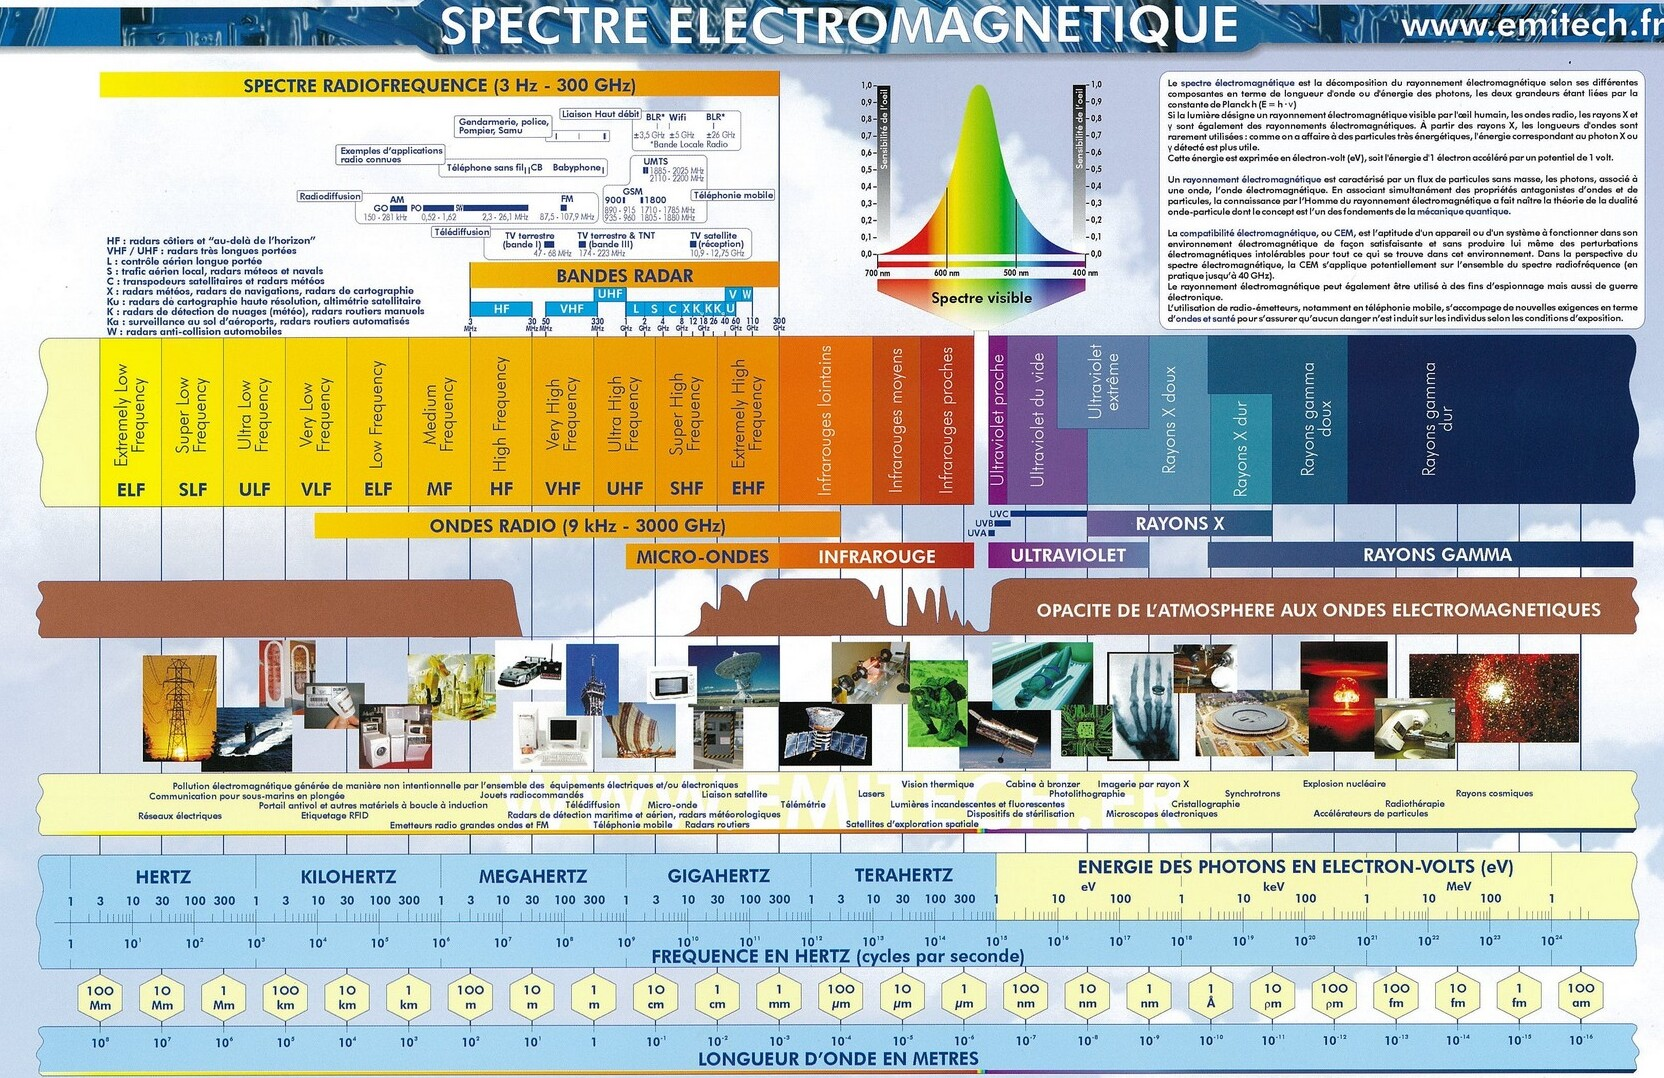
\includegraphics[height=\linewidth,angle=90]{ondes_EM_domaines.jpg}
\end{figure}

Les ondes électromagnétiques de différentes longueurs d'onde ont des applications très différentes. En effet, selon la longueur d'onde, le rayonnement pourra interagir avec différents composants de la matière (électrons, atomes, molécules ou objets macroscopiques). On distingue ainsi différents grands domaines de longueur d'onde (à connaître) :
\begin{itemize}
	\item Les ondes radio (de 10\,cm à 10\,km) utilisées pour les télécommunications ;
	\item Les micro-ondes (de 1\,mm à 10\,cm) qui interagissent avec les molécules d'eau notamment ;
	\item Les rayons infrarouges (de 1\,µm à 1\,mm) qui correspondent essentiellement au rayonnement de Planck des corps à température ambiante ;
	\item La lumière visible, entre 400 et 800\,nm ;
	\item Les rayons ultraviolets (de 1 à 400\,nm) qui peuvent interagir avec la structure électronique des atomes ;
	\item Les rayons X (10\,pm à 10\,nm) qui permettent de sonder les solides cristallins ;
	\item Les rayons gamma très énergétiques (en-dessous de 1\,\AA), notamment utilisés en radiothérapie.
\end{itemize}

\subsection{Représentation complexe}

Il est possible, comme en optique, d'adopter une représentation complexe des ondes planes progressives monochromatiques :
\begin{definition}
	Dans le cas d'une onde plane progressive monochromatique, on adopte une notation complexe pour le champ électrique et magnétique :
	\begin{equation}
		\underline{\vv E} = \underline{\vv{E_0}} e^{j(\omega t - \vv k \cdot \vv r)} \quad \mathrm{et} \quad \underline{\vv B} = \underline{\vv{B_0}} e^{j(\omega t - \vv k \cdot \vv r)}
	\end{equation}
	On a alors $\vv E = \Re\left(\underline{\vv E}\right)$ et $\vv B = \Re\left(\underline{\vv B}\right)$.
\end{definition}

Plusieurs propriétés mathématiques intéressantes s'appliquent alors, car on peut remarquer que les opérateurs divergence, rotationnel et gradient s'écrivent de la façon suivante :
\begin{equation}
	\begin{dcases}
		\div(\vv A) &= \vv \nabla \cdot \vv A \\
		\grad(A) &= \vv \nabla A \\
		\rot(\vv A) &= \vv \nabla \wedge \vv A
	\end{dcases}
\end{equation}
où l'on a noté $\vv \nabla = \left( \dfrac{\partial}{\partial x} ; \dfrac{\partial}{\partial y} ; \dfrac{\partial}{\partial z} \right)$.


\begin{capex}
	Exprimer l'action d'une dérivée temporelle, $\partial/\partial t$, et du vecteur $\vv \nabla$ sur le représentation complexe d'une onde plane progressive haromnique. En déduire que l'on peut remplacer les dérivées temporelles et les opérateurs vectoriels comme indiqué dans la propriété suivante.
\end{capex}

\begin{proposition}[Opérateurs vectoriels et représentation complexe]
	Pour une onde plane progressive monochromatique, les opérateurs peuvent se simplifier comme suit :
	\begin{align}
		\frac{\partial}{\partial t} &\leftrightarrow j \omega \times \\
		\div &\leftrightarrow j \vv k \cdot \\
		\grad &\leftrightarrow j \vv k \times\\
		\rot &\leftrightarrow j \vv k \wedge
	\end{align}
\end{proposition}

\subsection{Relation de dispersion}

\begin{capex}
	En utilisant l'équation de d'Alembert et la représentation complexe d'une onde électromagnétique, déterminer une relation entre la pulsation et le vecteur d'onde. Cette relation est appelée \textbf{relation de dispersion} et est à connaître par coeur.
\end{capex}

La relation de dispersion est la signature d'un type d'onde : elle est caractéristique de l'onde. La fréquence et la longueur d'onde sont en général des grandeurs mesurables (sauf dans le cas des très hautes fréquences) et la relation entre ces deux grandeurs est caractéristique d'une équation d'onde.

\subsection{Etude énergétique}

On s'intéresse désormais à l'énergie transmise par une onde plane progressive monochromatique. Pour cela, nous allons faire un bilan énergétique.

\begin{capex}
	On considère une onde plane progressive harmonique. Déterminer en fonction de $||\underline{\vv{E_0}}||$ et de $\vv k$:
	\begin{itemize}
		\item La densité volumique d'énergie électromagnétique $u_{\rm em}$ ;
		\item Le vecteur de Poynting $\vv \Pi$
	\end{itemize}
\end{capex}

On constate la propriété suivante, très importante :
\begin{proposition}
	Une onde plane progressive monochromatique, associée à une densité volumique d'énergie $u_{\rm em}$, et se propageant dans la direction $\vv u$, transporte l'énergie dans sa direction de propagation à la vitesse $c$ :
	\begin{equation}
		\vv \Pi = c u_{\rm em} \vv u
	\end{equation}
\end{proposition}

\section{Polarisation des ondes électromagnétiques}

\subsection{Relation de structure}

\begin{capex}
	Retrouver la relation de structure dans le cas des ondes planes progressives monochromatiques, et montrer qu'elle peut se mettre sous la forme :
	\begin{equation}
		\underline{\vv B} = \frac{\vv k \wedge \underline{\vv E}}{\omega}
	\end{equation}
	Cette relation est à connaître.
\end{capex}






\end{document}
